% 7장 어디로 번졌나. 0024

\section{어디로 번졌나}

토허제의 명분은 가격 안정이다. 규제 밖 단지로 수요가 옮겨 갔을 뿐이라면 규제는
문제를 푼 것이 아니라 \textbf{옮긴 것}이다. 선행연구 두 편이 `인근 지역 급등'을
보고했다\citep{lee2025, yang2025}.

\subsection{규제 밖이 세 층으로 있다}

이 자료에는 규제 밖이 세 층으로 있고 \textbf{층마다 사건이 다르다}(0024).

\begin{table}[htbp]
  \centering
  \caption{규제 밖의 세 층}
  \label{tab:spill-layers}
  \begin{tabular}{llp{6.5cm}}
    \toprule
    \textbf{층} & \textbf{사건} & \textbf{규제 밖에 무엇이 있나} \\
    \midrule
    1 같은 동 안 & 2025-02-13 해제 & 해제군 옆에 유지군 16개 단지가 남았다 \\
    2 옆 동 & 2020-06-23 지정 & 처치 4개 동에 11개 동이 맞닿는다 \\
    3 옆 구 & 2025-03-24 재지정 & 강남3구·용산이 막히고 4개 구가 남았다 \\
    \bottomrule
  \end{tabular}
\end{table}

\textbf{층 1이 이 연구의 특별한 조건이다.} 통상적인 파급효과 연구는 규제 지역과
인접한 비규제 지역을 비교하므로 두 지역이 원래 달랐을 가능성이 남는다. 2025년
2월 해제는 전면적이 아니라 부분적이어서 \textbf{같은 동 안에 규제 상태가 다른
단지가 공존}한다. 학군·교통·생활권이 물리적으로 동일하다.

맞닿은 동은 법정동 경계 다각형(467개)으로 뽑는다. 처치 4개 동 덩어리에 닿는 동이
14개이고, 창 안에 다른 계열로 지정된 동을 빼면 11개가 남는다.

\textbf{기준점을 명시하는 것이 이 장의 핵심이다.} 파급을 `처치동 대비'로 재면
처치동이 줄어든 것만으로도 옆 동이 늘어난 것처럼 보인다. 같은 자료·같은 창에
기준점만 바꿔 가며 사다리를 만들어 함께 싣는다.

\subsection{같은 동 안에서만 옮겨 갔다}

파급이 있으면 \textbf{규제가 바뀐 쪽과 안 바뀐 쪽의 부호가 반대}여야 한다. 한쪽이
늘 때 다른 쪽이 줄었으면 수요가 옮겨 간 것이고, 둘 다 줄었으면 같이 영향받은 것이다.

\begin{table}[htbp]
  \centering
  \caption{규제가 바뀐 쪽과 안 바뀐 쪽 (거래량). 층마다 사건이 다르다}
  \label{tab:spill-pairs}
  \begin{tabular}{llrr}
    \toprule
    \textbf{규제 밖이 어디에} & \textbf{사건} &
    \textbf{규제가 바뀐 쪽} & \textbf{안 바뀐 쪽} \\
    \midrule
    \textbf{같은 동 안} & 2025.2 해제 &
      해제군 $+80.6\%$ & 유지군 $\mathbf{-26.5\%}$ \\
    옆 동 & 2020.6 지정 &
      처치동 $-57.8\%$ & 맞닿은 동 $-9.0\%$ \\
    옆 구 & 2025.3 재지정 &
      강남3구·용산 $-82.3\%$ & 인접 4개 구 $+23.0\%$ (0.16) \\
    \bottomrule
  \end{tabular}
\end{table}

\textbf{같은 동 안에서는 옮겨 갔다.} 2025년 2월에 규제가 대부분 풀렸는데 16개
단지만 그대로 남았다. 풀린 쪽이 $+80.6\%$, \textbf{규제가 하나도 바뀌지 않은
유지군이 $-26.5\%$}다($p<0.001$, 먼 통제군 대비). 같은 동, 같은 학군, 같은 달인데
바뀐 것은 \textbf{옆 단지의 규제가 풀렸다는 것뿐}이다.

\textbf{옆 동으로는 가지 않았다.} 2020년 지정에서 맞닿은 동이 $-9.0\%$($p=0.088$)로
\textbf{늘어난 것이 아니라 같이 줄었다.} 공통지지 표본에서는 $-19.0\%$로 더
내려간다.

% 자동 생성 — scripts/build_tables.py. 손으로 고치지 않는다.
% 출처: output/results/12_spillover.json : 층2_고리별
\begin{table}[htbp]
  \centering
  \caption{2020-06 지정의 거리 고리별 효과. 서울 나머지 19개 구 대비.}
  \label{tab:spill-rings}
  \begin{tabular}{lrrrr}
    \toprule
    \textbf{고리} & \textbf{거래량 (\%)} & \textbf{$p$} & \textbf{가격 (\%)} & \textbf{$p$} \\
    \midrule
    R0 처치동 & -57.8 & $<0.001$ & -9.7 & $<0.001$ \\
    R1 맞닿은 동 & -9.0 & 0.088 & -5.0 & 0.001 \\
    R2 강남송파 비인접 & -2.4 & 0.664 & -1.5 & 0.269 \\
    R3 인접 4개구 & -10.4 & 0.055 & -0.7 & 0.459 \\
    \bottomrule
  \end{tabular}

  \begin{minipage}{\linewidth}\footnotesize
  \textit{주.} 어느 고리도 거래량이 양($+$)이 아니다. 거래가 옆 동으로 옮겨 간 흔적이 없다.
  \end{minipage}
\end{table}


\begin{figure}[htbp]
  \centering
  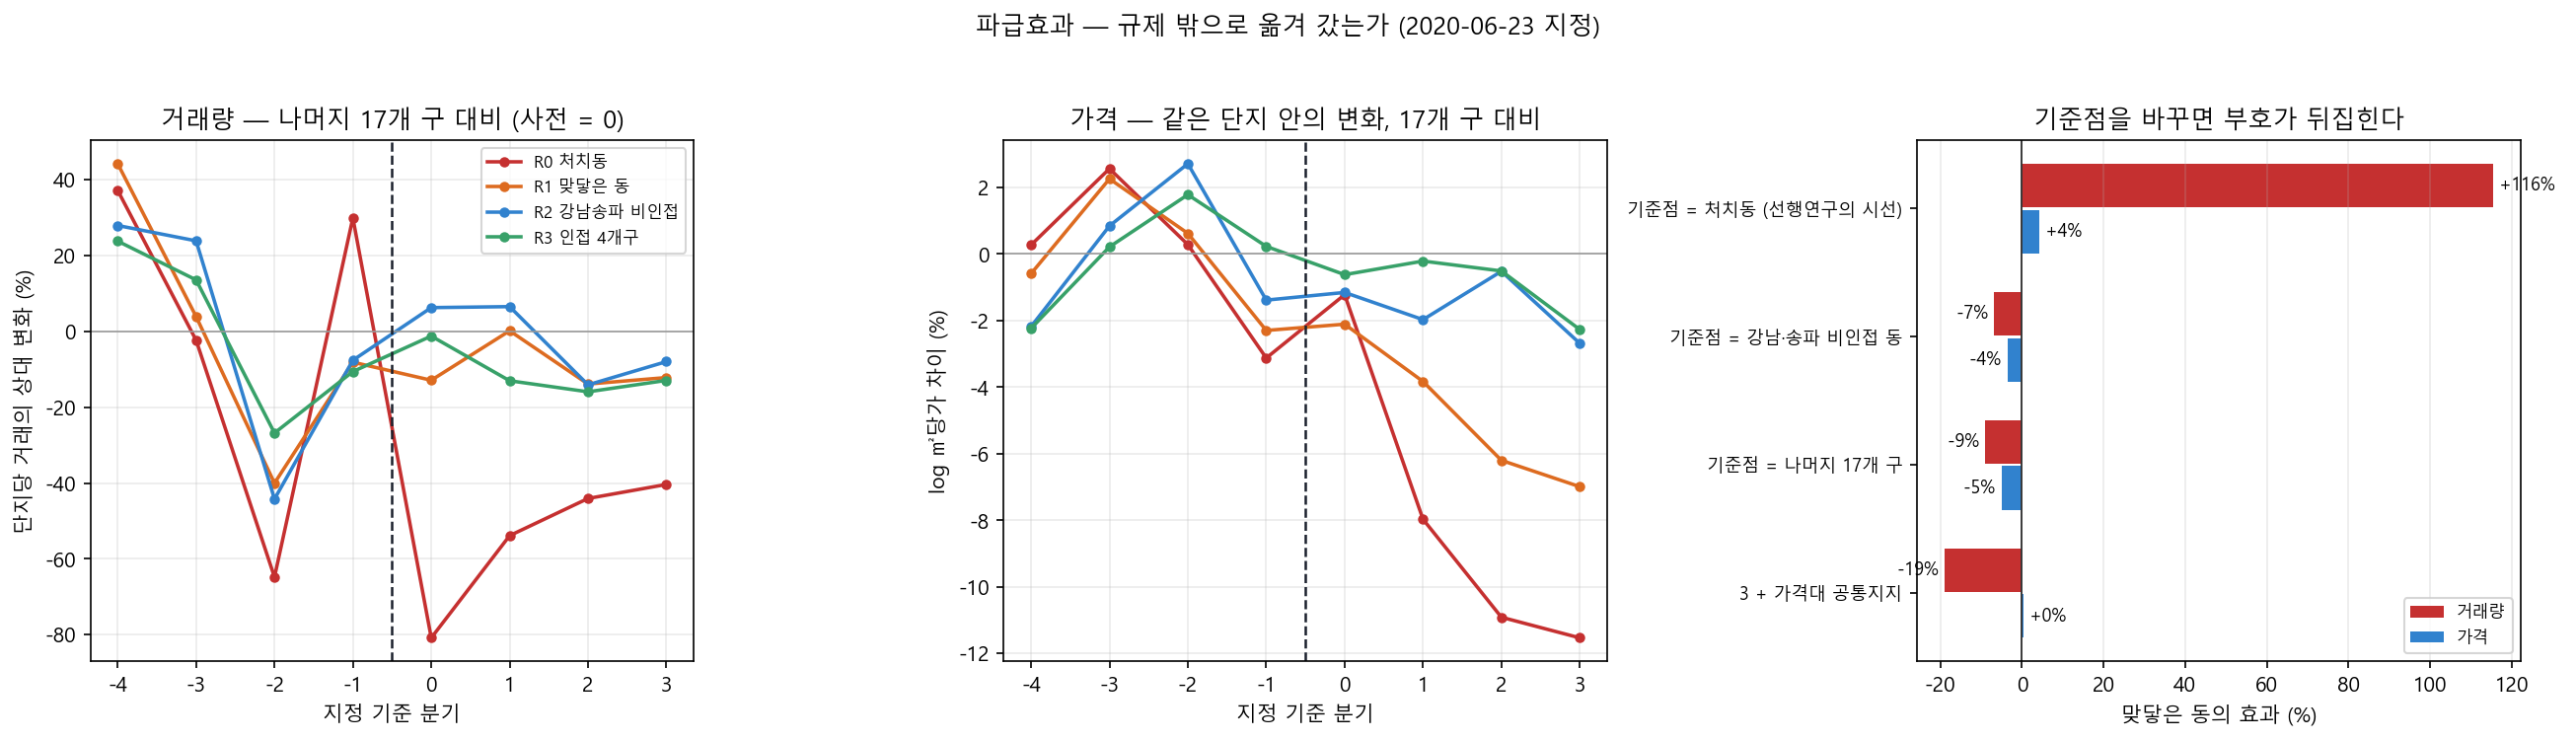
\includegraphics[width=\linewidth]{12_spillover.png}
  \caption{파급효과. 왼쪽 거리 고리별 거래량, 가운데 가격, 오른쪽 기준점을
           바꾸면 부호가 뒤집힌다.}
  \label{fig:spillover}
\end{figure}

\textbf{옆 구는 방향만 있다.} 2025년 재지정에서 인접 4개 구가 $+23.0\%$로 부호는
파급 방향이지만 $p=0.157$이다. 창이 5주로 짧고 늘리면 2025-06-27 대출 규제가
섞인다. \textbf{``인접 구로 넘어갔다''고 쓰지 않는다.} 같은 `인접 4개 구'가 2020년
사건에서는 $-10.4\%$로 부호가 반대인 것도 단정하지 말아야 할 이유다.

\textbf{여기서 `유의하지 않다'를 `효과가 없다'로 읽으면 안 된다.} 창이 5주라 검정력이
모자란 것인지 효과가 없는 것인지 가를 수 없다. \textbf{``확인할 수 없다''}로 쓴다.

\subsection{기준점을 바꾸면 부호가 뒤집힌다}

이 절이 7장에서 가장 중요하다. 아래 표는 \textbf{같은 맞닿은 동}이고 같은 자료,
같은 창, 같은 사양이다. \textbf{무엇과 견주는지만} 다르다.

% 자동 생성 — scripts/build_tables.py. 손으로 고치지 않는다.
% 출처: output/results/12_spillover.json : 사다리_맞닿은동
\begin{table}[htbp]
  \centering
  \caption{같은 자료, 같은 창, 같은 사양. 기준점만 바꿨다 (맞닿은 동).}
  \label{tab:spill-bench}
  \begin{tabular}{lrrrr}
    \toprule
    \textbf{기준점} & \textbf{거래량 (\%)} & \textbf{$p$} & \textbf{가격 (\%)} & \textbf{$p$} \\
    \midrule
    1. 기준점 = 처치동 (선행연구의 시선) & 115.5 & $<0.001$ & 4.3 & 0.111 \\
    2. 기준점 = 강남·송파 비인접 동 & -6.8 & 0.331 & -3.6 & 0.055 \\
    3. 기준점 = 나머지 19개 구 & -9.0 & 0.088 & -5.0 & 0.001 \\
    4. 3 + 가격대 공통지지 & -19.0 & 0.021 & 0.3 & 0.748 \\
    \bottomrule
  \end{tabular}

  \begin{minipage}{\linewidth}\footnotesize
  \textit{주.} $+115.5\%$ 는 옆 동이 늘어서가 아니라 처치동이 $-57.8\%$ 로 줄어서다. 선행연구가 보고한 `인근 급등' 이 이것이다.
  \end{minipage}
\end{table}


\textbf{처치동과 견주면 $+115.5\%$, 서울 나머지 19개 구와 견주면 $-9.0\%$다.}
맞닿은 동의 거래가 처치동보다 116\% 많아진 것은 \textbf{사실}이다. 그런데 그것은
옆 동이 늘어서가 아니라 \textbf{처치동이 57.8\% 줄어서}다. 분모가 반 토막 나면
가만히 있어도 상대적으로 두 배가 된다.

\subsection{선행연구의 `인근 급등'을 다시 읽는다}

\textbf{선행연구 두 편이 보고한 `인근 지역 급등'이 표~\ref{tab:spill-bench}의
첫 줄이다.} 계산이 틀린 것이 아니다. 기준점이 처치동일 뿐이다.

\begin{quote}
``토허제 때문에 인근이 급등했다''는 말은 \textbf{처치동을 기준으로 봤을 때만
참이다.} 기준점을 서울 전체로 한 칸만 옮기면 $-9.0\%$가 된다.
\end{quote}

처치동으로 같은 사다리를 놓으면 거래량은 기준점을 어떻게 바꿔도
$-57 \sim -64\%$다. \textbf{처치 효과는 기준점에 둔감하고 파급 효과는 민감하다.}
파급을 보고할 때 기준점을 밝히지 않으면 같은 자료에서 정반대 결론이 나온다는
것이 이 장의 방법론적 교훈이다.

그리고 \textbf{층을 가로질러 크기를 비교하지 않는다.} 창 길이부터 다르다 ---
2020년 사건은 $\pm$12개월, 2025년 사건은 전 13주·후 5주다. 어느 층의 숫자가 더
큰지 견주는 것은 뜻이 없다.
